
\vspace{-10ex}%
\rule{\textwidth}{0.3pt}
\vspace{5ex}
 % after-code

\textit{ 
This chapter describes the idea behind and the background to this project. A rough sketch of how the work is divided and the goals for this project is provided.
}
\vspace{5ex}

\section{Background}
This is not a new area of pruducts for Followit, different types of radio sending units have been made for over four decades now. 
With new and improved technology arriving each and every year new pruducts ought to be made to have the latest most efficient and effective systems. Every generation of a component will most likley have a smaller physical size, have more advanced features and draw less power then the previous one. Followit wants to make a new unit which implement all the new and improved technologies into a small, advanced product with low power consumption. 
Customers have been asking for a simple, small and cheap radio unit from the company to complement their more advanced and powerful products. With this type of product they could produce them in a larger number and gain new sale territories. By having such a small product it can be used in new areas that they never could before. The smaller the animal you want to track, the smaller equipment you could strap to them. This is one of the reasons that this product is so sought for in the buisness. 
\newline 
Most of the \gls{ic}'s are already chosen by the company, but there are no acctual implementations. The final version is supposed to work in different areas, both as a tracker for animals and also as a product for theft protection in cars a vehicles. This means that the design of the product needs versitality to work in all these different areas.  
Much consideration is taken to get the product both small and inexpencive. The cost of the PCB depends on the size, manufacturing and the numbers of layers. The rest of the cost comes down to the components, batteries and casing.    \\

\section{Project goals}
Followit wants to produce a VHF radio unit which have a powerful MCU for advanced programs and with some extra feautures that makes it possible to use the finished product in different areas and with different types of characteristics. The project involves a first test prototype and also a final version which is presented to the company as a finalised product ready for marketing and sales. To ensure proper functionallity of the prototype a test program is written to the system to test the connection and functionallity of all the components and acessebilities. 

Both the cost of the bare board and the components needs to be kept down.  This require some special attention to the board design, the manufacturing and component selection.
There will be a study of the ways of making the product both small and cheap at the same time. The problem formulation will be considering between making a prototype wich is tiny but have a high manufacturing cost and a inexpencive that have a bigger physical size. The procedure of finding a good balance between the two is explained later in further detail.

\section{Scope}
Main focus of this thesis is to create a PCB prototype that is tested and well designed and works as intended. Some of the coponents in the product are predefined but their implementation have to be done.
Extended test code is written to the product which includes tests for all the components in the circuit.  
The final PCB design will be delevered to the company for further programming and implemetation.
If case of time a casing for the product aswell as battery considerations wil be made.

\newpage
\section{Approach}
The idea that was presented to me was a half finished principle that i needed to understand and also expand with all the neccesary components that is not mentioned in this design. The initial work prior to this project can be seen in \autoref{anders_koppling}

\begin{figure}[H] 
	\centering 
	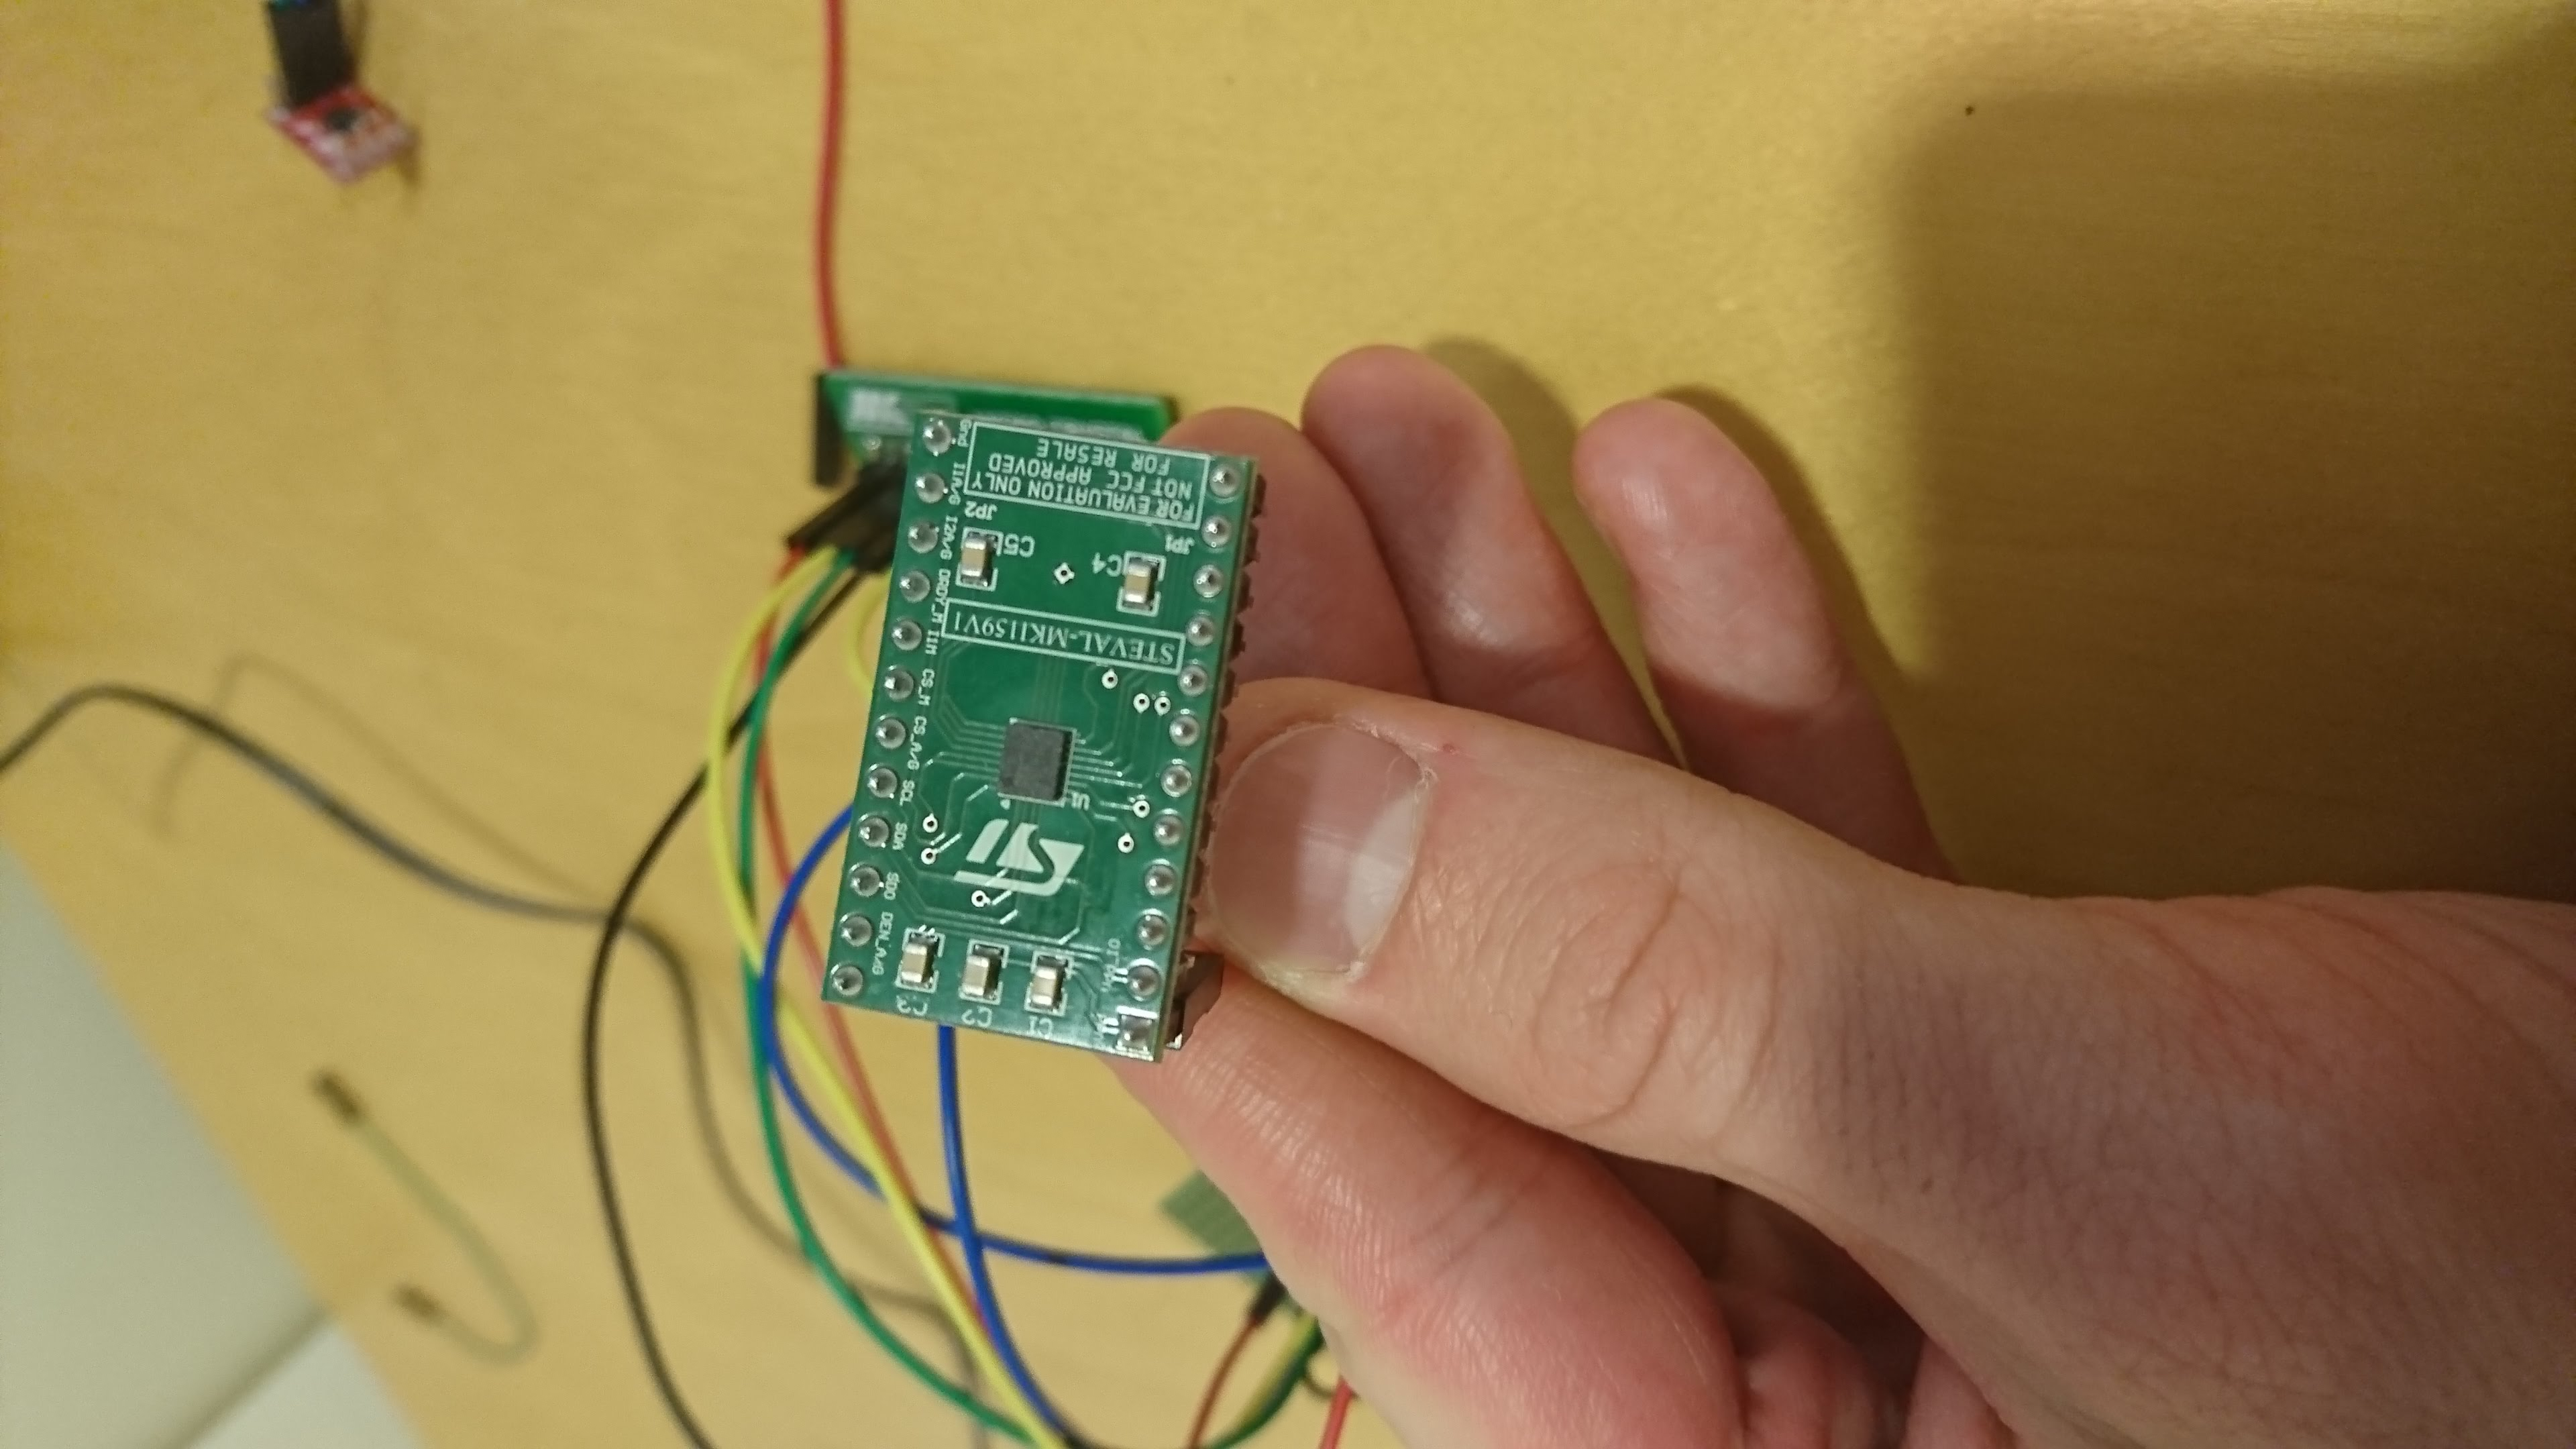
\includegraphics[width=.8\linewidth]{Figures/DSC_0103} 
	\captionsource{The initial schematics made by Followit}{Aurthor}
	\label{fig:anders_koppling} 
\end{figure} 

To get an understanding of all the parts and what there function are a list is constructed for a simple overview of the system.

\begin{itemize}[noitemsep]
	\item MCU - For processing data and connecting all the periferals together to a complete system.
	\item Accelerometer - Used for measuring movements. Important for knowing how much the device is moving or if lying still.
	\item Radio - All the communication to the outside world is done using radio transmissions. 
	\item RF switch - To switch between two low pass filter antennas from a single output.
	\item Real time Clock - The best way to keep an exact time, used for the system to keep track of the time even after one year of constant operation. 
	\item Hall switch - To turn on and off the device, a solution that is already used by the company.
	\item Programmable buck converter - To alternate the supply voltage for the system. 
	\item Logical inverter - To invert the signal for the programmable buck converter.
	\item LDO - Supply the radio oscillator.
	\item Other components - Two LED's, two oscillators, one for the processor and one for the radio module.
\end{itemize}


To get to the point of making the actual \gls{pcb} a thorough analyse of the components and their connections needs to be made. Firstly the datasheets are considered for an understanding of the component itself and the required connections for this particular implementation. Both power and data is crucial for operation and there might also be some peripherals connections and chip selection that needs to be considerd. \\
By writing a program the functions of each individual component can be tested. 

The processor used in this project comes from the PIC18 family of 8-bit processors produced by Microchip Technologies. This processor is a failry simpel unit, which makes it a bit more challanging to program. It doesen't have a buch of advanced libraries for example communication through SPI or I2C like some other commonly used processors. The process will therefore involve some close to hardware programming. A more thurough description of the processor will be described later in this report. The code language used for this project is C.

% Ha med?
\begin{comment}
In some cases the component needs to be initialized in a specific way or it needs some other special attention which might require additional connections than it firstly seemed.
With all the specified components connected together a program is made to show all the functions and that they work as intended. 
To ensure that each component on the PCB works and the prototype can be handed over to the software developers for a more advanced and optimized program. 
% Varför är den så bra?
\end{comment}

\thispagestyle{empty}